% !TEX program = xelatex
\documentclass[UTF8]{ctexrep}
\usepackage{xeCJK}
\setCJKmainfont[BoldFont=HiraginoSansGB-W3, ItalicFont=AdobeKaitiStd-Regular]{FZXSSJW--GB1-0}
\setCJKsansfont{HiraginoSansGB-W6}
\setCJKmonofont{FZLTXHK--GBK1-0}
\CTEXsetup[format+={\raggedright}]{section}

\usepackage{fontspec}
\setmainfont{TimesNewRomanPSMT}
\setsansfont{Verdana}
\setmonofont{CourierNewPSMT}

\usepackage{float}

\usepackage{geometry}
\geometry{a4paper,left=3cm,right=3cm,top=2.5cm,bottom=2.5cm}

\usepackage{fancyhdr}
\pagestyle{fancy}
\fancyhf{}
\chead{\itshape 现代密码学简介}
\rhead{\thepage}
\renewcommand\headrulewidth{0.6pt}

\makeatletter
\renewcommand\chapter{\if@openright\cleardoublepage\else\clearpage\fi
    \thispagestyle{fancy}% original style: plain
    \global\@topnum\z@
    \@afterindentfalse
    \secdef\@chapter\@schapter%
}
\makeatother

\renewcommand{\labelitemii}{$\circ$}

\usepackage{amsmath}
\usepackage{esvect}
\usepackage{bm}
\usepackage{upgreek}
\def \paral {/\!/}
\usepackage{mathtools}
\usepackage{amssymb}
\usepackage{extarrows}
\usepackage{mathrsfs}
\usepackage[amssymb]{SIunits}
\renewcommand{\epsilon}{\varepsilon}
\newcommand{\ext}{\displaystyle}
\newcommand{\arsinh}{\mathrm{arsinh}\,}
\newcommand{\arcosh}{\mathrm{arcosh}\,}
\newcommand{\artanh}{\mathrm{artanh}\,}
\newcommand{\dif}{\mathop{}\!{}\mathrm{d}}
\newcommand{\ic}{\mathrm{i}}
\newcommand{\Tr}{\mathrm{T}}
\newcommand{\ke}{\mathrm{k}}
\newcommand{\p}{\mathrm{p}}
\newcommand{\Z}{\mathbb{Z}}

\def\mathbm#1{{\bm #1}}
\def\vec#1{\vv{\bm #1}}
\def\xvec#1#2{\vv{{\bm #1}_{#2}}}
\def\yvec#1#2{\vv{{\bm #1}^{#2}}}
\def\abs#1{\left| #1 \right|}
\def\pth#1{\left( {#1}\right)}
\def\brack#1{\left[ {#1}\right]}
\def\brace#1{\left\{ {#1} \right\}}
\def\E#1#2{{\mathrm{E}_{#1}\left({#2}\right)}}
\def\D#1#2{{\mathrm{D}_{#1}\left({#2}\right)}}
\def\GF{\mathrm{GF}}
\renewcommand{\rem}{{\bfseries Remark}}

\usepackage{amsthm}

\newtheorem{Definition}{\hspace{2em}定义}[chapter]
\newtheorem{theorem}{\hspace{2em}定理}[chapter]

\usepackage[framemethod=tikz]{mdframed}
\newenvironment{prove}{\begin{mdframed}[backgroundcolor=gray!10,roundcorner=8pt]}{\end{mdframed}}

\usepackage{hyperref}
\hypersetup{pdfauthor={张曙},
pdftitle={现代密码学简介},
hidelinks
}
\begin{document}
\tableofcontents
\thispagestyle{fancy}
\chapter{绪论}
\section{什么是密码学}
如果我们要求一个从未接触过密码学的人处理一段文字,把这段文字尽可能地加密,让别人无法破解。那么,大多数人在深思熟虑之后,总能提出一些加密算法。这时候,一般人的思路可能会有几个方向。\par
有的人的方向是把这段文字中的字母之间通过各种复杂的运算进行组合。比如说,把要加密的文字中每两个字母在字母表中的位置进行相加,形成密码。比如说,``cryptography''中,``cr''变成了$3+18=21$, ``yp''变成了$25+16=41$, ``cryptography''对应的密码就是``214135252133''。但这样的密码,显然忽略了一点:密码的可解密性。我们之所以要进行加密,是为了安全地传递信息。但接收信息者必须要有解密的方法。但这种加密方式则没有对应的解密方法。所以说,这不是一个合格的加密方式。\par
这时,足够聪明的人,则考虑到了解密的方法。他们想出了一些类似于古代使用的加密方法。比如说,著名的凯撒密码:把一段由英文字母组成的语句,每个字母都在字母表中往后移3个位置。``veni vidi vici''也就变成了``yhql ylgl ylfl''. 这种密码的解密方法,也就是每个字母在字母表中向前移动3个位置。当问起这种密码体制里最重要的是什么,大部分人都会说是加密算法。如果把加密算法告诉了别人,那这种密码就相当于被破解了。\par
如果进而问起一个密码体制的组成,大部分人的回答,就是加密算法。也许有些自诩比普通人聪明一点的人,还会加上一个解密算法,也就是,将处理过后的密码变为正常文字的算法。如果用$m$代表要被加密的文字,$c$代表被加密出来的密码,$\mathrm{E}()$代表加密算法,$\mathrm{D}()$代表解密算法,那么大多数人理解的密码学,本质就是以下这两个式子:
\begin{gather*}
    c=\mathrm{E}\pth{m}\\
    m=\mathrm{D}\pth{c}
\end{gather*}

\subsection{密钥}
但是,我们考虑一下实际的情况。根据我们之前的常识,会发现,如果要用密码来传递信息,首先通信的双方必须要在一个安全信道中传递一些额外的信息。比如说,告诉接收者加密的方式,或者更直接地,告诉接收者解密算法。不存在一种加密的方式,能不事先通过安全信道传递信息,而使得只有接收者能够解密。那么,为了使通信更加安全,通信双方对安全信道的使用应该尽可能少。如果Alice和Bob使用凯撒密码进行通信,而Alice事先在安全信道中要对Bob说“我的这种加密方式是把一段由英文字母组成的语句,每个字母都在字母表中往后移3个位置。”这段话是如此之长,而如果考虑是在战场上,由通信员用摩尔斯电码发送,那么花费的这么长的时间显然是不合理的。再者,现代的通信方式一般都是把信息编码成二进制进行传递,那么,相比把一段话编码成二进制,不如找一些数字来代表这个密码。在我们的这段思想博弈中,一个重要的概念呼之欲出。\par
拿凯撒密码为例,在其加密算法中,还有一个关键的量:3. 试想,如果通信双方Alice和Bob, Alice在场的所有人她用的是凯撒密码的加密方式加密她的话,又在安全信道中告诉Bob``4'', 意味着她使用的凯撒密码里,是将每个字母在字母表的位置上向后移动4个位置。那么,即使在场有人能偷听到Alice给Bob的密码,也无法破解Alice想说的是什么,只有掌握了规则“向后移动4个位置”的Bob, 才能正确地破解密码。\par
如果还是按照之前的说法,一个密码体制包括加密算法和解密算法,那么向后移动3个位置的凯撒密码和向后移动4个位置的凯撒密码,就成了两个密码体制。但是,这两种加密方式是极其类似的,差别也就只在于一个向后移动3个位置,一个向后移动4个位置。我们对于这些密码的研究,也许也就十分类似。因此,把这两种加密方式归类为同一种密码体制,似乎是更好的选择。因此,\textbf{密钥}就应运而生了。所谓密钥,我们可以粗略地理解成加密算法、解密算法中的参数,也就是我们之前说的3、4. 通过一个密码体制通信的双方,需要首先在保密信道中确定密钥。而一个密码体制,也就可以由加密算法、解密算法和密钥构成。因此,如果以$k$代表密钥,那么之前的式子就变成了
\begin{gather*}
    c=\E{k}{m}\\
    m=\D{k}{c}
\end{gather*}

这也就是现在通用的密码学。\par
那么我们思考几个问题:在一次加密通信过程中,加密算法和解密算法中使用的密钥是否必须要相同?密钥是否只能是一个数?可不可以没有密钥?\par
针对第一个问题,确实存在某些高端的技巧,使得加密算法和解密算法使用的密钥是不同的。事实上,在密码学领域中,根据加密算法和解密算法使用的密钥是否相同,人们将加密方式分为对称加密与非对称加密,分别对应使用同一密钥和使用不同密钥。非对称加密方式也许难以理解,我们也会在充分学习对称加密后再介绍非对称加密。所以,我们接下来讨论的对称加密过程中,请大家记住,加密算法和解密算法使用的是相同的密钥。\par
此外,对于对称加密算法,密钥也并不一定是一个数。比如说,加密算法
\[\E{a, b}{m}=am+b\]
其密钥为$\pth{a, b}$, 但我们仍认为其使用单一密钥,也就是说,把$\pth{a, b}$看作一个密钥。\par
此外,可不可能不存在密钥呢?确实有这样的密码体制,但这样却也十分不安全。比如说,加密算法
\[\mathrm{E}\pth{m}=m\]
就是一个无密钥的加密算法。
\section{密码体制的基本要素}
根据之前的讨论,我们就可以得出一个密码体制的基本要素:
\begin{itemize}
    \item 明文空间$\mathcal{M}$\par
    所有可以被加密算法加密的元素组成的集合,加密算法的定义域。明文空间的元素叫做明文$m\in\mathcal{M}$.\par
    例如,在凯撒密码中,明文空间就为所有由英文字母组成的字符串。
    \item 密文空间$\mathcal{C}$\par
    所有可以由加密算法输出的元素组成的集合,加密算法的值域。密文空间的元素叫做密文$c\in\mathcal{C}$.\par
    我们需要注意到的是,这里的值域,可以理解成二元函数$\mathrm{E}\pth{k, m}$的值域。比如说,对于加密算法
    \[\E{k}{m}=m^2+k^2\]
    其密文空间为$[0, +\infty)$而非$[k^2, +\infty)$.
    \item 密钥空间$\mathcal{K}$\par
    所有密钥组成的集合。密钥空间的元素叫做密钥$k\in\mathcal{K}$.\par
    在非对称加密中,密钥空间分为加密密钥空间和解密密钥空间。
    \item 加密算法$\E{k}{m}$\par
    根据密钥生成的特定算法,将明文转化为密文。
    \item 解密算法$\D{k}{c}$\par
    根据密钥生成的特定算法,将密文转化为明文。\par
    对于对称加密算法,也就是只使用一个密钥的加密体制,解密算法与加密算法满足
    \[\D{k}{\E{k}{m}}=m\]
\end{itemize}

在我们讨论密码体制的一些性质时,密钥生成算法有时也是必要的。什么是密钥生成算法呢?回忆之前Alice和Bob的例子,凭什么Alice选择的密钥是4而不是25呢?这就涉及到了密钥生成算法。在这个例子中,密钥生成算法就是Alice自己想到哪个密钥就输出哪个密钥。但是,从严格意义上来讲,密钥生成算法是一种概率算法。所谓概率算法,就是在算法的步骤中涉及到了某些概率。比如说,在某个密钥生成算法中,在$(0, 1)$中等概率随机生成一个数$t$, 而生成的密钥$k$满足
\[
    k=\begin{cases}1&t\in\pth{0.5, 1}\\0&t=0.5\\-1&t\in\pth{0, 0.5}\end{cases}
\]

这就是一个典型的概率算法。其特点就是在两次运行中输出的结果不一定相同。\par
因此,我们称一个加密方案包含三个要素:加密算法$\mathrm{E}$, 解密算法$\mathrm{D}$, 密钥生成算法$\mathrm{G}$. 根据定义,我们可以说,一个密码体制由一个加密方案$\pth{\mathrm{E}, \mathrm{D}, \mathrm{G}}$及一个明文空间$\mathcal{M}$完全定义。\par
因此,Alice和Bob的一次加密通信的过程包括:
\begin{enumerate}
    \item Alice根据密钥生成算法$\mathrm{G}$生成密钥$k\in\mathcal{K}$.
    \item Alice通过安全信道将$k$告诉Bob.
    \item Alice将想要传达的明文$m\in\mathcal{M}$根据加密算法加密成密文$c=\E{k}{m}$告诉Bob.
    \item Bob根据之前Alice告诉自己的$k$、密文$c$及解密算法得出明文$m=\D{k}{c}$
\end{enumerate}

那么,在一个密码体制中,哪个最重要呢?是不是之前我们说的加密算法呢?这里,就不得不提Kerckhoffs原则。用现代的语言来说,Kerckhoffs原则阐述的是:
\begin{quote}
    提倡安全性不能建立在对算法的保密上。
\end{quote}

也就是说,我们如果要证明一个加密体制的安全性,不能指望算法的保密性。我们应默认加解密算法可以被所有人知道(事实上也确实如此)。也就是说,真正值得保密的,是密钥。如果潜在的敌手获得密钥,那么根据公开的解密算法,那么他就可以从窃得的密文中获得明文。
\section{经典密码}
\subsection{基础概念}
我们讨论了密码体制的基本要素之后,就可以介绍一些经典的密码,让大家更好地理解这些术语了。\par
值得指出的是,这些密码都是古代欧洲人的研究成果,当时并没有如今“数字化”的概念。因此,这些密码,都是针对拉丁字母进行的加密。因此,我们首先要引入一些概念:\par
函数$C\pth{m}$将拉丁字母$m$映射到它在字母表中的位置上,比如$C(a)=1, C(z)=26$. 函数$I\pth{n}$将位于$1$和$26$之间的数字映射到字母表中相应位置的拉丁字母上,比如$I(1)=a, I(26)=z$.\par
在讨论经典密码时,一些极其基础的数论记号及知识可以让我们更加方便、更加简洁地叙述、理解这些经典密码。\par
我们用$\gcd\pth{a, b}$表示$a$与$b$的最大公因数。\par
用$a\bmod{b}$表示整数$a$除以$b$后的余数(取值范围为$0$到$b-1$), 比如说$15\bmod{6}=3, 12\bmod{6}=0, \pth{-4}\bmod{6}=2$.\par
若$a\bmod{b}=0$, 即$a$能整除$b$, 我们则记为$a\mid b$. 如$2\mid 4, 3\nmid 4$.\par
若$\pth{a-b}\mid c$, 我们则称$a$与$b$模$c$同余,记作$a\equiv b\pmod{c}$. 如$16\equiv 23\pmod{7}$.\par
对于整数$a, b$, 若存在整数$c$使得$ac\equiv 1\pmod{b}$, 则称$c$为$a$在模$b$时的逆,记作$a^{-1}$. 并非所有的整数都有逆,如在模$4$的情况下,整数$2$就没有逆。对于整数$a, b$, 在模$b$时$a$存在逆的充分必要条件为$\gcd\pth{a, b}=1$.
\subsection{单表代换密码}
单表代换密码的典型,就是凯撒密码。如果用我们上述的记号来表示凯撒密码的过程,那么如果设明文为字符串``$m_1m_2\cdots m_n$'',密文为字符串``$c_1c_2\cdots c_n$'', $m_i, c_i$均代表一个拉丁字母。凯撒密码的加密算法
\begin{equation}
    c_i=\E{}{m_i}=C\pth{\pth{I\pth{m_i}+3}\bmod{26}}
\end{equation}

解密算法
\begin{equation}
    m_i=\D{}{c_i}=C\pth{\pth{I\pth{c_i}-3}\bmod{26}}
\end{equation}

它通过对字母表中每个字母进行固定的代换,得到密码。单表替换密码则是凯撒密码的推广,引入了密钥。从数学意义上,可以作如下定义:\par
设明文为字符串``$m_1m_2\cdots m_n$'',密文为字符串``$c_1c_2\cdots c_n$'', $m_i, c_i$均代表一个拉丁字母。如果把整数对$\pth{a, b}$作为密钥,其中$a\neq 0$, 那么其加密算法
\[c_i=\E{a, b}{m_i}=C\pth{\pth{aI\pth{m_i}+b}\bmod{26}}\]

解密算法
\[m_i=\D{a, b}{c_i}=C\pth{\pth{a^{-1}\pth{I\pth{c_i}-b}}\bmod{26}}\]
其中$a^{-1}$为$a$模$26$的逆。\par
事实上,如果我们令$n_i=I\pth{m_i}, q_i=I\pth{\E{a, b}{m_i}}, e_i=I\pth{\E{a, b}{m_i}}, d_i=I\pth{\D{a, b}{\E{a, b}{m_i}}}$, 那么
\[q_i\equiv an_i+b\pmod{26}\]

故
\begin{align*}
    d_i&\equiv a^{-1}\pth{q_i-b}\\
    &\equiv a^{-1}\pth{an_i+b-b}\\
    &\equiv n_i\pmod{26}
\end{align*}

也就是说,
\[I\pth{\D{a, b}{\E{a, b}{m_i}}}\equiv m_i\pmod{26}\]

故
\[\D{a, b}{\E{a, b}{m_i}}=m_i\]

这也就证明了这个加密算法是正确的算法。\par
让我们不要再纠结于繁琐的数学符号,我们来从直观上看一看这个加密算法。任意取一个密钥,比如说,$a=3, b=7$, 就会对应的生成一张加密表和解密表:
\begin{table}[H]
    \centering
    \caption{$a=3, b=7$时的加密表}
    \begin{tabular}{c|c|c|c|c|c|c|c|c|c|c|c|c|c}\hline
        明文&a&b&c&d&e&f&g&h&i&j&k&l&m\\
        密文&h&k&n&q&t&w&z&c&f&i&l&o&r\\\hline
        明文&n&o&p&q&r&s&t&u&v&w&x&y&z\\
        密文&u&x&a&d&g&j&m&p&s&v&y&b&e\\\hline
    \end{tabular}
\end{table}
\begin{table}[H]
    \centering
    \caption{$a=3, b=7$时的解密表}
    \begin{tabular}{c|c|c|c|c|c|c|c|c|c|c|c|c|c}\hline
        密文&a&b&c&d&e&f&g&h&i&j&k&l&m\\
        明文&p&y&h&q&z&i&r&a&j&s&b&k&t\\\hline
        密文&n&o&p&q&r&s&t&u&v&w&x&y&z\\
        明文&c&l&u&d&m&v&e&n&w&f&o&x&g\\\hline
    \end{tabular}
\end{table}

那么我们根据这张表,就可以很快地进行加密和解密的工作了。\par
我们再回到之前所说的加密体制的基本要素:其明文空间$\mathcal{M}$为由拉丁字母组成的任意长度的字符串组成的集合,密文空间$\mathcal{C}=\mathcal{M}$. 密钥空间$\mathcal{K}=\brace{\pth{a, b}\mid a, b\in \Z, \gcd\pth{a ,26}=1}$(这里$\gcd\pth{a, 26}=1$的条件是因为解密算法中要求$a$模$26$的逆存在。).
\subsection{单表代换密码的破解}
上述的单表代换密码看似十分安全,但是如果用来加密由拉丁字母组成的用语言逻辑形成的一句话时,却有一个致命的弱点。虽然这些密码不会直接暴露明文,但却会暴露明文中各个字母出现的频率。我们知道,在任何一门由字母组成的语言文字中,每个字母出现的频率在语句十分长时是趋向于一个定值的。比如说,在英文中,有一个著名的短语:``ETAOIN SHRDLU''. 这个短语是英文中出现频率最高的12个字母,从高到低排列。根据这些频率,就可以找到破解这种密码的方法。利用这个原理,有两种最常用的方法:频率分析法与巧合指数法。
\subsubsection{频率分析法}
假设利用单表代换密码加密的语言为英文,那么根据统计学家的知识,英文字母出现的频率从高到低依次是``ETAOIN SHRDLU''. 如果我们可以统计出一个相当长的密文中各个字母出现的频率,那么极有可能出现频率最高的字母对应的就是明文中的``E''. 这就是频率分析法的基本思想。
\subsubsection{巧合指数法}
巧合指数法的想法非常直接:对于一段文字,任意取两个字母,这两个字母相同的概率称为巧合指数$\mathrm{IC}$。可以证明,对于一段长度为$N$的文字,共有$c$个字母,每个字母出现的次数为$n_i$, $i=1, 2, \ldots, c$. 那么巧合指数的值为
\begin{equation}
    \mathrm{IC}=\frac{\ext\sum_{i=1}^cn_i\pth{n_i-1}}{N\pth{N-1}}
\end{equation}

如果这段文字充分长,那么我们有
\begin{equation}
    \frac{\ext\sum_{i=1}^cn_i\pth{n_i-1}}{N\pth{N-1}}\approx\frac{\ext\sum_{i=1}^cn_i^2}{N^2}
\end{equation}

如果记$\ext p_i=\frac{n_i}{N}$表示第$i$个字母在这段文字中出现的频率,那么
\begin{equation}
    \mathrm{IC}\approx\sum_{i=1}^cp_i^2
\end{equation}

而我们先前提到,统计学家已经统计出在英文文本中各个字母出现的频率,因此,带入上述式子,可以得出英文文本的巧合指数$\mathrm{IC}\approx 0.0686$. \par
接着我们统计加密过后的密文的巧合指数,假设密钥为$k$, 我们对$k=0, 1, \ldots, 25$依次去试,如果出现了解密后的文本的巧合指数接近于$0.0686$, 就说明这个$k$有很大可能是密钥。
\subsection{多表代换密码}
为了进一步提高安全性,古代的人们想到也许一张表并不足够安全,不妨使用多张表。因此,多表代换密码应运而生。\par
假设一共有$t$张加密表,人们是怎么做的呢?从明文的第一个字符开始,第一个字符使用第一张加密表进行加密,第二个字符使用第二张加密表进行加密,以此类推,第$t$个字符使用第$t$张加密表进行加密。到了第$t+1$个字符,则又回到第一张加密表进行加密。用数学的语言怎么叙述这件事呢?\par
对于明文字符串$M=m_1m_2\cdots m_n$, 我们要求其长度满足$n=tp$. 我们将明文字符串等分成$p$个列向量$M_1, M_2, \ldots, M_p$, 其中$M_i=\pth{m_{p(i-1)+1}, m_{p(i-1)+2}, \ldots, m_{p(i-1)+t}}^{\mathrm{T}}$. 对密文字符串$C$也作同样的划分$C_1, C_2, \ldots, C_p$. 取密钥为$\pth{A, B}$, 其中矩阵$A$为$t\times t$的可逆矩阵,且满足$\gcd\pth{\abs{A}, 26}=1$, $B$为$t$维列向量。\par
那么多表代换密码的加密算法为
\begin{equation}
    C_i=\E{A, B}{M_i}=C\pth{\pth{AI\pth{M_i}+B}\bmod{26}}
\end{equation}

解密算法为
\begin{equation}
    M_i=\D{A, B}{C_i}=C\pth{\pth{A^{-1}I\pth{C_i-B}}\bmod{26}}
\end{equation}

其中$A^{-1}$满足
\[A^{-1}A\bmod{26}=\pth{\begin{array}{cccc}1&0&\cdots &0\\0&1&\cdots&1\\\vdots&\vdots&\ddots &\vdots\\0&0&\cdots&1\end{array}}\]

我们可以用一个具体的例子来理解这些抽象的公式:\par
假设我们一共有三张表,分别使用密钥为$\pth{1, 1}, \pth{3, 3}, \pth{5, 7}$的单表替换密码生成。明文字符串$M=m_1m_2\cdots m_n$的长度$n=3p$. 我们将其等分为$p$个列向量$M_1, M_2, \ldots, M_p$, 其中$M_i=\pth{m_{p(i-1)+1}, m_{p(i-1)+2}, m_{p(i-1)+3}}^{\mathrm{T}}$. 对于密文字符串$C$也作同样的划分$C_1, C_2, \ldots, C_p$. 取
\[A=\pth{\begin{array}{ccc}1&0&0\\0&3&0\\0&0&5\end{array}}, B=\pth{\begin{array}{c}1\\3\\7\end{array}}\]
为密钥。\par
那么其加密算法为
\begin{align*}
    \pth{\begin{array}{c}c_{p(i-1)+1}\\c_{p(i-1)+2}\\c_{p(i-1)+3}\end{array}}=C_i&=\E{A, B}{M_i}=\pth{\begin{array}{ccc}1&0&0\\0&3&0\\0&0&5\end{array}}M_i+\pth{\begin{array}{c}1\\3\\7\end{array}}\bmod{26}\\
    &=\pth{\begin{array}{c}m_{p(i-1)+1}+1\\3m_{p(i-1)+2}+3\\5c_{p(i-1)+3}+7\end{array}}\bmod{26}
\end{align*}

其解密算法为
\[M_i=\D{A, B}{C_i}=\pth{\begin{array}{ccc}1&0&0\\0&9&0\\0&0&21\end{array}}\pth{C_i-\pth{\begin{array}{c}1\\3\\7\end{array}}}\bmod{26}\]

那么我们可以看到,从明文的第一个字符开始,每隔三个字符的第一个字符使用的加密方法为$c_{p(i-1)+1}=\pth{m_{p(i-1)+1}+1}\bmod{26}$, 第二个字符使用的加密方法为$c_{p(i-1)+2}=\pth{3m_{p(i-1)+2}+3}\bmod{26}$, 第三个字符使用的加密方法为$c_{p(i-1)+3}=\pth{5m_{p(i-1)+3}+7}\bmod{26}$. 这也就是我们设计多表代换密码的原意。\par
我们发现,在上述例子中,密钥里的$A$似乎有许多$0$的位置。但是,我们之前在数学上严格定义多表代换密码的时候,并没有要求这些位置一定要是$0$. 事实上,这些位置如果不是$0$,就意味着密文中特定位置的字符并不是由明文中对应位置的字符确定,而是明文中对应位置与前后位置的字符一起确定。这也是可行的。
\subsection{一次一密}
之前我们说道,单表代换密码可以根据每个字母出现的频率来破解,其实多表代换密码的破解也很类似。那么,有没有什么方法能使密文不显示明文中每个字母出现的频率呢?一次一密的方法就是答案。\par
为了加密某个长度为$n$的字符串,我们取另一个长度为$n$的字符串作为密钥。所得的密文就是明文每个字符在字母表中的位置与密钥每个字符在字母表中的位置相加。由密文得到明文也就是密文中每个字符在字母表中的位置与密钥每个字符在字母表中的位置相减。\par
这种方式之所以称为一次一密,是因为同一串密钥只能使用一次。试想如果有人窃得了用同一串密钥加密的两个密文$C_1, C_2$, 将这两个字符串中的每个字符按其在字母表中的位置相减,那么如果出现$0$, 那么对应位置就就有可能是出现频率比较高的几个字母。当然,更严谨的论证可以用之后提到的概率论的方式证明。\par
最后,值得一提的是,现代使用的量子加密中,最常用的加密机制就是一次一密。
\section{加密系统的安全性}
为了从数学上定义加密系统的安全性,我们必须引入一些和概率有关的定义。这时,请回忆一下之前定义的加密方案$\pth{\mathrm{E}, \mathrm{D}, \mathrm{G}}$. 其中,$\mathrm{E}$代表加密算法,$\mathrm{D}$代表解密算法,$\mathrm{G}$代表密钥生成算法。此外,还有明文空间$\mathcal{M}$, 密文空间$\mathcal{C}$, 密钥空间$\mathcal{K}$.\par
对于$m\in\mathcal{M}$, $M$为表示明文的随机变量,用$\Pr\brack{M=m}$表示明文为$m$的概率。这一定义看似难以理解,为什么明文会出现概率呢?从某种意义上,可以理解成假想的敌手在没有任何信息的情况下猜测明文的概率。比如说,在没有任何信息的情况下,一个敌手可能会假定明文为``attack tomorrow''或``don't attack''. 且敌手认为明文为``attack tomorrow''的概率为$0.6$, 明文为``don't attack''的概率为$0.4$.\par
对于$k\in\mathcal{K}$, $K$为表示密钥值的随机变量,用$\Pr\brack{K=k}$表示随机算法$\mathrm{G}$输出$k$的概率。(由常识可知,$K$与$M$是独立的)\par
对于$c\in\mathcal{C}$, $C$为表示密文的随机变量,用$\Pr\brack{C=c}$表示密文为$c$的概率。由于密文是完全由明文及密钥确定的,所以我们可以知道:
\begin{equation}
    \Pr\brack{C=c}=\sum_{c=\E{k}{m}} \Pr\brack{M=m}\Pr\brack{K=k}
\end{equation}

我们定义完善保密(perfect secrecy):
\begin{Definition}
对于明文空间为$\mathcal{M}$的加密方案$\pth{\mathrm{E}, \mathrm{D}, \mathrm{G}}$,若对$\mathcal{M}$上的任何概率分布,任何明文$m\in\mathcal{M}$、任何密文$c\in\mathcal{C}$且$\Pr\brack{C=c}$有
\begin{equation}
    \Pr\brack{M=m\mid C=c}=\Pr\brack{M=m}
\end{equation}
则称加密方案$\pth{\mathrm{E}, \mathrm{D}, \mathrm{G}}$是完善保密。
\end{Definition}

用一句通俗的话来讲,就是敌手在窃取密文之后并不会对明文有任何知识。而用概率论的说法,则是随机变量$M$与$C$是独立的。\par
我们可以通过一些概率论上的技巧,证明“一次一密”的加密方式是完善保密。\par
但是,完善保密也有其胶柱鼓瑟之处:
\begin{theorem}
若明文空间为$\mathcal{M}$的加密方案$\pth{\mathrm{E}, \mathrm{D}, \mathrm{G}}$是完善保密,则
\begin{equation}
    \abs{\mathcal{K}}\geq\abs{\mathcal{M}}, \abs{\mathcal{C}}\geq\abs{\mathcal{M}}
\end{equation}
\end{theorem}

如果用通俗的语言解释上述定理,则是说:要想实现完善保密,则密钥至少要和明文一样长,而密文则也至少要和明文一样长。\par
我们之前说过,要想实现加密通信,通信双方一定要事先在安全信道中沟通密钥。如果密钥至少和明文一样长,那与其沟通密钥,不如直接把明文告诉对方了。此外,生成的密文也至少和明文一样长,这也是十分浪费通信资源的手段。因此我们可以看到,完善保密确实是一个难以实现的目标。\par
对于感兴趣的同学,我们可以介绍一个判断一个加密方案是否是完善保密的简单方法,即香农定理:
\begin{theorem}
对于明文空间为$\mathcal{M}$的加密方案$\pth{\mathrm{E}, \mathrm{D}, \mathrm{G}}$, 若$\abs{\mathcal{K}} = \abs{\mathcal{M}} = \abs{\mathcal{C}}$, 则当且仅当下列条件成立时,此方案是完善保密加密:
\begin{enumerate}
    \item 由$\mathrm{G}$产生的任意密钥$k\in\mathcal{K}$的概率都是$\ext\frac{1}{\abs{\mathcal{K}}}$
    \item 对任意明文$m\in\mathcal{M}$和任意密文$c\in\mathcal{C}$, 只存在唯一的密钥$k\in\mathcal{K}$使得$c=\E{k}{m}$.
\end{enumerate}
\end{theorem}

关于完善保密,我们的讨论就告一段落。最后,介绍一下对加密系统安全性的分类。\par
对加密系统安全性的分类,现在主流学界习惯上以敌手的算力及时间进行划分:
\begin{itemize}
    \item 无条件安全\par
        如果假设攻击者在无限资源的前提下,也无法破译加密算法,就认为相应的密码体制是无条件安全的。\par
        这里的无限资源,可以包括无限算力和无限时间。\par
        可以把无条件安全的加密方式理解成完美加密。
    \item 计算安全\par
        使用目前最好的方法攻破它所需要的计算远远超出攻击者的计算资源水平,则可以定义这个密码体制是计算安全的。\par
        比如说,如果要破解某个加密算法需要用当今最好的计算机连续工作一万年,那么我们就可以认为这个密码体制是计算安全的。
    \item 可证明安全\par
        如果破译某加密算法的困难性与破解某些困难数学命题的困难性相同(如大整数的因数分解),则可以定义这个密码体制是可证明安全的。 
\end{itemize}

值得指出的是,关于加密系统的安全性,尽管我们使用日常的语言叙述的这些概念,但这些概念实际上都是有严格的数学定义的。鉴于我们目前的数学 水平有限,在这里引入这些数学概念是不适合的。因此,我们仅从感性上理解这些概念即可。
\chapter{流密码}
\section{数学上的基本概念}
从这章开始,我们就不再拘泥于古代的加密拉丁字母的加密方式,而开始转向数字化。我们知道,在现代科技中,密码学最常应用的领域就是计算机领域,而计算机领域则是由二进制的$0, 1$串构成。因此,在接下来的讨论中,我们都将明文空间及密文空间看作由$0$和$1$构成的二进制串组成的集合。\par
因此,为了接下来能更顺畅地进行关于流密码的讨论,这里先介绍一些数学上关于这方面的基础知识。
\subsection{$\GF\pth{2}$上的加法与乘法}
由于我们讨论的仅是$0$和$1$及它们的运算, 因此,我们定义一个有限域$\GF\pth{2}=\brace{0, 1}$. \par
有限域$\GF\pth{2}$上的加法被定义成逻辑上的异或,也可以理解成模$2$加法。以下为$\GF\pth{2}$上的加法表:
\begin{table}[H]
    \centering
    \caption{$\GF\pth{2}$上的加法表}
    \begin{tabular}{c|cc}\hline
        $+$&0&1\\\hline
        0&0&1\\
        1&1&0\\\hline
    \end{tabular}
\end{table}

如果我们定义一个集合中元素$a$的加法逆元$-a$满足
\[a+\pth{-a}=\pth{-a}+a=0\]

则$\GF\pth{2}$上的加法逆元表为:
\begin{table}[H]
    \centering
    \caption{$\GF\pth{2}$上的加法逆元表}
    \begin{tabular}{c|cc}\hline
        $a$&0&1\\\hline
        $-a$&0&1\\\hline
    \end{tabular}
\end{table}

而$\GF\pth{2}$上的减法则可以定义成与加法逆元的加法,即
\begin{equation}
    a-b=a+\pth{-b}
\end{equation}

$\GF\pth{2}$上的乘法则被定义成了逻辑上的与。以下为$\GF\pth{2}$上的乘法表:
\begin{table}[H]
    \centering
    \caption{$\GF\pth{2}$上的乘法表}
    \begin{tabular}{c|cc}\hline
        $\cdot$&0&1\\\hline
        0&0&0\\
        1&0&1\\\hline
    \end{tabular}
\end{table}

根据上述的定义,我们可以得出以下$\GF\pth{2}$上常用的运算规则:
\begin{itemize}
    \item 
        \begin{equation}
            \forall x\in\GF\pth{2}, x+x=0
        \end{equation}
    \item 
        \begin{equation}
            \forall x, y\in\GF\pth{2}, x-y=y-x=x+y
        \end{equation}
    \item 
        \begin{equation}
            \forall x\in\GF\pth{2}, x\cdot x=x
        \end{equation}
\end{itemize}
\subsection{$\GF\pth{2}$上的多项式}
此外,还有一个我们未曾接触过的知识:$\GF\pth{2}$上的多项式。为此,不妨先介绍一下多项式理论。\par
对于表达式
\begin{equation}
    a_nx^n+a_{n-1}x^{n-1}+\cdots +a_1x+a_0=\sum_{i=0}^na_ix_i
\end{equation}

我们称其系数为$a_0, a_1,\ldots, a_n$. 其系数集$S$为$a_0, a_1,\ldots ,a_n$的取值范围。当$a_n\neq 0$时,称该多项式为$S$上的$n$次多项式。比如说,如果其系数的取值仅限于$0$和$1$, 则称这个多项式为$\GF\pth{2}$上的多项式。\par
值得指出的是,我们研究多项式理论时,多项式在我们眼中仅仅是一个表达式,我们并不需要去对每一个$x$的取值进行多项式的求值。它就相当于一个集合的元素,一个多项式就是一个最小的单位。其加、减、乘、除就应该像我们定义复数集那样重新地进行定义。也就是说,我们通过定义来确定多项式$f+g=h$, 而不是通过$\forall x, h(x)=f(x)+g(x)$来定义多项式之和。尽管结果确实如此,但这应该理解为自洽的定义,而非推导。\par
\subsubsection{多项式的加法}
两个多项式之和的多项式的系数,等于其对应系数之和。即:\par
若$m\geq n$, 则
\begin{equation}
    \sum_{i=0}^ma_ix^i+\sum_{j=0}^nb_jx^j=\sum_{k=0}^n\pth{a_k+b_k}x^k+\sum_{i=n+1}^ma_ix^i
\end{equation}
其中$a_k+b_k$的加法应理解成系数集$S$上的加法。\par
用更形象的方法来说,我们不妨考虑实数集上的多项式$f=x^2+1$与$g=x^3+x^2$, 那么其和我们可以类似于小学时的竖式来计算:
\begin{table}[H]
    \centering
    \begin{tabular}{ccrcrcr}
        $f$&$=$&&&$x^2$&$+$&$1$\\
        $g$&$=$&$x^3$&$+$&$x^2$&$+$&$1$\\\hline
        $f+g$&$=$&$x^3$&$+$&$2x^2$&$+$&$2$
    \end{tabular}
\end{table}

但是,我们这里也需要注意到刚刚说的,$a_k+b_k$的加法应理解成系数集$S$上的加法。比如说还是刚刚的两个多项式,但其在$\GF\pth{2}$上的加法为:
\begin{table}[H]
    \centering
    \begin{tabular}{ccrcrcr}
        $f$&$=$&&&$x^2$&$+$&$1$\\
        $g$&$=$&$x^3$&$+$&$x^2$&$+$&$1$\\\hline
        $f+g$&$=$&$x^3$&&&&
    \end{tabular}
\end{table}

这里$2x^2$与$2$之所以不见了,是因为在$\GF\pth{2}$上,$1+1=0$.
\subsubsection{多项式的减法}
类似于多项式的加法的定义,两个多项式之差的系数,等于其对应系数之差。在$\GF\pth{2}$上的多项式之差的例子:
\begin{table}[H]
    \centering
    \begin{tabular}{ccrcrcr}
        $f$&$=$&&&$x^2$&$+$&$1$\\
        $g$&$=$&$x^3$&$+$&$x^2$&$+$&$1$\\\hline
        $f-g$&$=$&$x^3$&&&&
    \end{tabular}
\end{table}

这里是由于$\pth{0-1}x^3=\pth{0+1}x^3=x^3$, $\pth{1-1}x^2=0$, $1-1=0$.
\subsubsection{多项式的乘法}
我们可以形式上地用乘法分配律进行计算,并且约定$x^ix^j=x^{i+j}$. 下面演示一下$\GF\pth{2}$上多项式的乘法运算:
\begin{align*}
    &\pth{x+1}\pth{x+1}\\
    =&xx+\pth{1+1}x+1\\
    =&x^2+1
\end{align*}
注意到在$\GF\pth{2}$上,$\pth{1+1}x=0$.\par
同时,我们记$f^n=f\cdot f^{n-1}$.
\subsubsection{多项式的整除}
对于多项式$f$和$g$, 如果存在多项式$h$, 使得$f=gh$, 则称$g$整除$f$, 记作$g\mid f$, 同时$\ext \frac{f}{g}=h$.\par
注意这仍是在系数集$S$上的。比如说,在$\GF\pth{2}$中,我们有
\[\pth{x^2+1}\mid\pth{x+1}^2\]

此外,若一个多项式$f$是不可约的,则说明不存在两个多项式$g, h$, 使得$gh=f$且$g, h$的次数均小于$f$的次数。
\subsubsection{$\GF\pth{2}$上的常用等式}
加法交换律
\begin{equation}
    f+g=g+f
\end{equation}

加法结合律
\begin{equation}
    \pth{f+g}+h=f+\pth{g+h}
\end{equation}

乘法交换律
\begin{equation}
    fg=gf
\end{equation}

乘法结合律
\begin{equation}
    \pth{fg}h=f\pth{gh}
\end{equation}

乘法对加法的分配律
\begin{equation}
    f\pth{g+h}=fg+fh
\end{equation}

等比数列求和公式:对于多项式$f$和$g\neq 1$
\begin{equation}
    f+gf+fg^2+\cdots +fg^{n-1}=\sum_{i=0}^{n-1}fg^{i}=\frac{f-fg^{n}}{1-g}
\end{equation}
\subsubsection{总结}
在$\GF\pth{2}$这个有限域上的运算和我们在实数集上的运算很不一样,所以在后文中我们应该着重注意运算是定义在$\GF\pth{2}$上的还是定义在实数集上的。同时,我们也该清楚定理叙述的是多项式之间的关系还是值之间的关系。
\section{流密码的基本概念}
之前我们讲到“一次一密”的加密方式是完善保密,同时,“一次一密”的缺点也十分显著:密钥过长。那么,有什么办法能规避这样的缺点呢?事实上,“一次一密”的加密方式之所以是完善保密的,最重要的一点是每次密钥的字符串是随机生成的。通过之前讲的香农定理我们可以知道,每个密钥字符串生成的概率均是相等的。如果我们可以降低一点这种随机性的要求,那也许就能实现短密钥+强保密的目标。\par
为此,我们引入\textbf{伪随机数序列}的概念。由于这个概念的严格定义需要高超的概率论及算法知识,我们只需要感性地理解伪随机数序列为一种,由确定的算法产生的(即相同的初始条件下的输出是相同的),与真随机数序列性质几乎一样的序列。\par
那么\textbf{流密码}的工作模式可以简单地看作:对于给定长度的一串明文$M=m_1m_2\cdots m_n$, 我们输入密钥$k$, 通过某种算法产生一个同样长度的伪随机序列$Z=z_1z_2\cdots z_n$作为密钥流, 输出结果$Y=y_1y_2\cdots y_n$为明文串与伪随机序列按位异或的结果$y_i=m_i\oplus z_i$. 根据之前在$\GF\pth{2}$上的讨论,解密算法也是将密文串与密钥流进行按位异或,即$m_i=y_i\oplus z_i$.\par
根据上述的定义,流密码与一次一密的区别就在于,在与明文串进行按位异或的过程中,一次一密使用的是真随机序列,流密码使用的是伪随机序列。如何能使伪随机序列的表现足够像真随机序列,则是流密码安全性的关键。因此,对流密码的研究,主要就在于产生伪随机序列的算法上。\par
设$f(k, \sigma_i)$为一个能产生伪随机序列的算法,其中$k$为输入的密钥,$\sigma_i$为当前时刻系统的状态。在每个时刻,$f(k, \sigma_i)$输出一个伪随机数,同时系统状态改变为$\sigma_{i+1}$. 常把一个用于加密算法的伪随机序列称为\textbf{密钥流},产生伪随机序列的算法称为\textbf{密钥流产生器}。\par
那么流密码的过程可以理解为:如果设明文为二进制串$X=x_1x_2\cdots x_n$, 密钥为$k$. 在初始状态下,输入$x_1$和$k$, 密钥流生成器根据当前的状态输出一个伪随机数$z_1$, 输出密文$y_1=x_1\oplus z_1$. 接着输入$x_2$, 密钥流生成器根据当前的状态输出一个伪随机数$z_2$, 输出密文$y_2=x_2\oplus z_2$. 以此类推。
\section{密钥流产生器}
之前在讲到密钥流生成器的时候,我们提到了系统当前的状态$\sigma_i$. 这里的状态,是根据当前的输入和输出而变化的。每输入一个数,密钥流生成器每输出一个数,当前系统的状态就发生了变化。之后会介绍一些具体的例子让大家更加理解“系统的状态”的含义。在这里,我们将流密码分为同步流密码和自同步流密码。如果密钥流生成器中的状态与输入的明文有关,则称为\textbf{自同步流密码},反之则称为\textbf{同步流密码}。我们接下来讨论的都是同步流密码。\par
为了生成近似真随机的伪随机序列,常见的密钥流产生器由线性部分和非线性部分组合。但是,并非所有的密钥流产生器都是这种工作原理。还有别的能产生伪随机序列密钥流的方法,如RC4算法等。
\subsection{密钥流产生器的线性部分}
\subsubsection{LFSR}
根据上述的讨论,密钥流产生器应有两个功能:输出密钥流与更新系统状态。密钥流产生器的线性部分也有两个功能:输出中间的过渡字符,并且更新系统状态。所谓中间的过渡字符,意思是该部分的输出并非作为最终输出的伪随机数,而是一个中间用于之后计算的数。\par
常见的处理方法为:系统的状态$\sigma_i=a_{n, i}a_{n-1, i}\cdots a_{1, i}$由$n$个二进制数构成。在启动之前,具有初始状态$a_{n, 0}a_{n-1, 0}\cdots a_{1, 0}$. 之后,每次的输出$b_i$为
\begin{equation}
    b_i=a_{1, i-1}
\end{equation}

而状态更新的方法为
\begin{equation}
    a_{j, i}=\begin{dcases}a_{j+1, i}&1\leq j\leq n-1\\f\pth{a_{1, i-1}, a_{2, i-1}, \ldots, a_{n, i-1}}&j=n\end{dcases}
\end{equation}

其中\textbf{反馈函数}$f\pth{a_{1, i-1}, a_{2, i-1}, \ldots, a_{n, i-1}}$是一个$\GF\pth{2}$上的线性函数。即:
\begin{align}
    a_{n, i}&=f\pth{a_{1, i-1}, a_{2, i-1}, \ldots, a_{n, i-1}}\notag\\
    &=c_na_{1, i-1}+c_{n-1}a_{2, i-1}+\cdots +c_1a_{n, i-1}\\
    &=\sum_{k=1}^nc_{n+1-k}a_{k, i-1}
\end{align}
其中$c_k\in\GF\pth{2}$, 即$c_k$的取值为$0$或$1$. 这些数字都是固定的,由密钥流产生器本身决定。而这里的加法、乘法运算均为$\GF\pth{2}$上的运算。\par
我们通过一个例子来熟悉:\par
设初始状态为$110$, 反馈函数$f(a_{3, i}, a_{2, i}, a_{1, i})=a_{3, i}+a_{1, i}$. 则我们可以通过下表来了解这个线性部分的输出:
\begin{table}[H]
    \centering
    \begin{tabular}{c|c|c|c|c|c|c|c|c|c}\hline
        $i$&0&1&2&3&4&5&6&7&$\cdots$\\\hline
        $f(a_3, a_2, a_1)$&1&0&1&0&0&1&1&1&$\cdots$\\\hline
        $a_3$&1&1&0&1&0&0&1&1&$\cdots$\\\hline
        $a_2$&1&1&1&0&1&0&0&1&$\cdots$\\\hline
        $a_1$&0&1&1&1&0&1&0&0&$\cdots$\\\hline
        $b$&&0&1&1&1&0&1&0&$\cdots$\\\hline
    \end{tabular}
\end{table}

其输出序列就为$011101\quad 011101\cdots$.\par
我们由上面的表可以发现,从每一列来看,随着$i$的递增,上一行的数会传给下一行的数。这似乎是某种线性寄存器的工作形式。因此,我们称密钥流产生器的线性部分为一个\textbf{线性反馈移位寄存器}(Linear Feedback Shift Register, LFSR). 若其状态具有$n$个二进制数字,且$c_n\neq 0$, 则称其为$n$级LFSR.
\subsubsection{LFSR的输出序列}
如果设$B=b_1b_2\cdots b_i\cdots $表示LFSR的输出序列,则由上述的讨论也可以知道
\begin{equation}
    \pth{b_{i+1}b_{i+2}\cdots b_{i+n}}=\pth{a_{1, i-1}a_{2, i-1}\cdots a_{n, i-1}}
\end{equation}

我们还可以认为,每一个$b_i$都可以代表LFSR的一个状态。那么,由于LFSR的一个状态中有$n$个二进制数,故一个LFSR至多有$2^n$种状态。如果称状态$\sigma=00\cdots 0$为零状态,下面我们证明:零状态的下一个状态是零状态,任何非零状态的下一个状态均不是零状态。
\begin{prove}
前半句话显然,设$\forall 1\leq j\leq n, a_{j, i}=0$. 对于$j\leq n-1$, $a_{j, i+1}=a_{j+1, i}=0$. 而
\[a_{n, i}=c_na_{1, i-1}+c_{n-1}a_{2, i-1}+\cdots +c_1a_{n, i-1}=0\]

对于后半句话,若某个非零状态$\sigma_i=a_{n, i}a_{n-1, i}\cdots a_{1, i}$的下一个状态为零状态,则由定义可知,$\forall 2\leq j\leq n, a_{j, i}=a_{j-1, i+1}=0, a_{n, i+1}\neq 0$. 且
\[0=a_{n, i+1}=c_na_{1, i}+c_{n-1}a_{2, i}+\cdots +c_1a_{n, i}=c_na_{1, i}\]

又由于$c_n\neq 0$, 故$a_{1, i}=0$矛盾。
\end{prove}

由上述讨论可知,一个LFSR中的状态,至多$2^n-1$个之后即达成循环。也就是说,一个LFSR产生的序列,周期至多为$2^n-1$. 
\begin{Definition}
    我们称由LFSR产生的周期为$2^n-1$的序列为一个$m$序列。
\end{Definition}
\subsubsection{$m$序列相关定理}
上述的讨论中,我们提到,反馈函数
\[a_{n, i}=c_na_{1, i-1}+c_{n-1}a_{2, i-1}+\cdots +c_1a_{n, i-1}\]
中的$c_1, c_2,\ldots ,c_n$由LFSR本身决定。因此:
\begin{Definition}
    我们称$\GF\pth{2}$上的多项式
\begin{equation}
    p(x)=1+c_1x+\cdots +c_{n-1}x^{n-1}+c_nx^n
\end{equation}
为LFSR的特征多项式。\par
对于LFSR生成的一个序列$a_1a_2\cdots a_n\cdots$, 称幂级数
\begin{equation}
    A\pth{x}=\sum_{i=1}^{\infty}a_ix^{i-1}
\end{equation}
为该序列的生成函数。\par
对于使用给定的LFSR, 由于初始状态不同而产生的所有$2^n-1$个非零序列构成的集合记作$G\pth{p\pth{x}}$.
\end{Definition}

下面叙述一个在证明中很有用的定理:
\begin{theorem}
设LFSR的特征多项式$p(x)=1+c_1x+\cdots +c_{n-1}x^{n-1}+c_nx^n$, $A\pth{x}$为$G\pth{p(x)}$中任意序列$\brace{a_n}$的生成函数,则对于$\GF\pth{2}$上的多项式$p(x)$和$A(x)$, 满足
\begin{equation}
    A(x)=\frac{\phi(x)}{p(x)}
\end{equation}

其中
\begin{equation}
    \phi(x)=\sum_{i=1}^n\pth{c_{n-i}x^{n-i}\sum_{j=1}^ia_jx^{j-1}}
\end{equation}
\end{theorem}

我们可以对$\phi(x)$进行展开:
\begin{align*}
    \phi(x)&=\sum_{i=1}^n\pth{c_{n-i}x^{n-i}\sum_{j=1}^ia_jx^{j-1}}\\
    &=\sum_{i=1}^n\pth{\sum_{j=1}^ic_{n-i}a_jx^{n-i+j-1}}\\
    &\xlongequal{k=n-i+j-1}\sum_{i=1}^n\sum_{k=n-i}^{n-1}c_{n-i}a_{k-n+i+1}x^k
\end{align*}

因此,我们可以发现,$\phi(x)$的次数不超过$n-1$.
\begin{Definition}
对于$\GF\pth{2}$上的多项式$p(x)$, 若$p(x)\mid x^p-1$, 则称最小的$p$为$p(x)$的阶。
\end{Definition}

一个与之相关的定理是:
\begin{theorem}
设$p(x)$是$n$次不可约多项式,其阶为$m$. 则$\forall \brace{a_n}\in G\pth{p(x)}$, $\brace{a_n}$的周期为$m$.
\end{theorem}
\begin{Definition}
若$n$次不可约多项式$p(x)$的阶为$2^{n}-1$, 则称$p(x)$是本原多项式。
\end{Definition}

下面叙述的是最关键的一个定理:
\begin{theorem}
设$\brace{a_n}\in G\pth{p(x)}$, 则$\brace{a_n}$为$m$序列的充要条件是$p(x)$是本原多项式。
\end{theorem}
\subsubsection{LFSR是伪随机数产生器}
为了叙述本节的定理,我们引入两个概念:
\begin{Definition}
对于序列$\brace{a_n}$, 长度最大为$n$的连续的0或者1称为一个长度为$n$的0游程或1游程。\par
对于$\GF\pth{2}$上周期为$2$的序列$\brace{a_n}$, 称其异相关函数为
\begin{equation}
    R\pth{\tau}=\frac{1}{T}\sum_{k=1}^T\pth{-1}^{a_k}\pth{-1}^{a_{k+\tau}}, 0<\tau\leq T-1
\end{equation}
\end{Definition}

之前我们提到的伪随机数序列,我们在这里给出一种定义方法:
\begin{Definition}
对于周期序列$\brace{a_n}$, 其为伪随机序列的条件为
\begin{enumerate}
    \item 在序列的一个周期内,$0$与$1$的个数至多相差1.
    \item 在序列的一个周期内,长为$i$的游程占游程总数的$\ext\frac{1}{2^i}$, 且其中0游程与1游程个数相等。
    \item 该序列的异相关函数是个常数。
\end{enumerate}
\end{Definition}

那么我们可以证明,一个$n$长$m$序列是这种意义下的伪随机序列。
\subsubsection{LFSR密码的破译}
在本节介绍的破译方式中,值得强调的是,敌手是知道LFSR为$n$级,且敌手获得了一串长度为$2n$的明密文对。\par
假设敌手获得的明密文对为$x_1x_2\cdots x_{2n}$和$y_1y_2\cdots y_{2n}$, 其需要破译的是LFSR的特征多项式的系数$c_1, c_2,\ldots, c_n$. 那么由于在$\GF\pth{2}$上
\[y_i=x_i+z_i\]
其中$z_i$为产生的密钥流的第$i$位。\par
故在$\GF\pth{2}$上
\[x_i+y_i=x_i+x_i+z_i=z_i\]

从而敌手就获得了一段长度为$2n$的密钥流$z_1z_2\cdots z_{2n}$.\par
如果记
\begin{equation}
    S_i=\pth{z_{i+1}, z_{i+2}, \ldots, z_{i+n}}^{\mathrm{T}}, i=0, 1,\ldots, n-1
\end{equation}

且
\begin{equation}
    X=\pth{S_0,S_1,\ldots, S_{n-1}}
\end{equation}

故根据表达式
\begin{equation}
    z_{n+i}=c_nz_{i}+c_{n-1}z_{i+1}+\cdots +c_{1}z_{i+n-1}
\end{equation}

可得:
\begin{equation}
    \pth{z_{n+1}, z_{n+2},\ldots, z_{2n}}=\pth{c_n, c_{n-1}, \cdots ,c_{1}}X
\end{equation}

而我们可以证明$X$是可逆的。故
\begin{equation}
    \pth{c_n, c_{n-1}, \cdots ,c_{1}}=\pth{z_{n+1}, z_{n+2},\ldots, z_{2n}}X^{-1}
\end{equation}
\subsection{密钥流产生器的非线性部分}
由上述的讨论我们可以发现,线性的密钥流产生器产生的密钥流一定是周期的。而周期较短的密钥流则相当于一种多表代换密码,相对容易破解。因此,只有加上非线性的部分来处理,才能提高安全性。\par
密钥流产生器的非线性部分的主要工作是接受一个或多个LFSR的输入,以非线性的方式,输出密钥流。\par
我们综合判定一个输出密钥流的优劣,可以从两个方面:周期和线性复杂度。周期越长,线性复杂度越高的密钥流越安全。周期我们可以直接衡量,而线性复杂度我们该如何衡量呢?我们称一个序列的线性复杂度为生成该序列的最短LFSR的级数。即若该序列周期$T$满足$2^{n-1}-1<T\leq 2^{n}-1$, 则该序列的线性复杂度为$n$.
\subsubsection{Geffe序列生成器}
Geffe序列生成器接受三个LFSR的输入,其输入分别为序列$\brace{a_n^{(1)}}, \brace{a_n^{(2)}}, \brace{a_n^{(3)}}$.\par
其输出序列$\brace{b_k}$可以表示为
\begin{table}[H]
    \centering
    \begin{tabular}{c|c}\hline
        $a_k^{(2)}$&$b_k$\\\hline
        $0$&$a_k^{(3)}$\\\hline
        $1$&$a_k^{(1)}$\\\hline
    \end{tabular}
\end{table}

若$\brace{a_n^{(1)}}$, $\brace{a_n^{(2)}}$和$\brace{a_n^{(3)}}$的周期分别为$2^{n_1}-1$, $2^{n_2}-1$和$2^{n_3}-1$且$n_1, n_2, n_3$两两互素,则$\brace{b_k}$的周期为$\pth{2^{n_1}-1}\pth{2^{n_2}-1}\pth{2^{n_3}-1}$, 线性复杂度为$\pth{n_1+n_3}n_2+n_3$
\subsubsection{JK触发器}
JK触发器接受两个LFSR的输入,其输入分别为序列$\brace{a_n^{(1)}}, \brace{a_n^{(2)}}$.\par
其输出序列$\brace{b_k}$可以表示为
\begin{table}[H]
    \centering
    \begin{tabular}{c|c|c}\hline
        $a_k^{(1)}$&$a_k^{(2)}$&$b_k$\\\hline
        $0$&$0$&$b_{k-1}$\\\hline
        $0$&$1$&0\\\hline
        $1$&$0$&0\\\hline
        $1$&$1$&$\overline{b_{k-1}}$\\\hline
    \end{tabular}
\end{table}

若$\brace{a_n^{(1)}}$和$\brace{a_n^{(2)}}$的周期分别为$2^n-1$和$2^m-1$且$m, n$互素,$a_0^{(1)}+a_0^{(2)}=1$, 则$\brace{b_k}$的周期为$\pth{2^n-1}\pth{2^m-1}$
\subsubsection{钟控序列生成器}
钟控序列接受两个LFSR的输入,其输入分别为序列$\brace{a_n^{(1)}}, \brace{a_n^{(2)}}$. 前一个序列控制后一个序列的时钟周期$n_k$.\par
其输出序列$\brace{b_k}$可以表示为
\begin{table}[H]
    \centering
    \begin{tabular}{c|c|c}\hline
        $a_k^{(1)}$&$n_k$&$b_k$\\\hline
        $0$&$n_{k-1}$&$a_{n_k}^{(2)}$\\\hline
        $1$&$n_{k-1}+1$&$a_{n_k}^{(2)}$\\\hline
    \end{tabular}
\end{table}

若$\brace{a_n^{(1)}}$和$\brace{a_n^{(2)}}$的周期分别为$p_1$和$p_2$, 且记$\ext w=\sum_{i=0}^{p_1-1}a_i^{(1)}$, 则$\brace{b_k}$的周期为$\ext\frac{p_1p_2}{\gcd\pth{w, p_2}}$. 若$p_1=2^m-1, p_2=2^n-1$, 则其线性复杂度为$n\pth{2^m-1}$.
\chapter{分组密码}
\section{设计密码系统的方法}
我们之前提到如凯撒密码、多表代换密码等经典密码的时候,讲到了破解这些密码的一种方法,就是利用英文中每个字母出现的频率不同。一次一密的方法可以抵御这种破解,原因是对于明文中的每个字符,其移位都是随机的,因此在密文中完全没有明文中字母出现的频率的信息。但是,一次一密的成本又太高,我们有没有什么办法,能尽可能地掩盖在密文中出现的字母频率的信息,来抵御这种频率攻击呢?香农给出了一种解决方法。
\subsection{扩散与混淆}
所谓扩散,指的是如果我们改变明文中的一个字符,加密得到的密文中的多个字符也会得到改变;如果我们改变密文中的一个字符,解密得到的明文中的多个字符也同样会得到改变。因此,明文中一个字符的信息被“扩散”到密文中的多个字符。因此,实现扩散的方法,就可以是用明文中的多个字符去生成密文中的一个字符。\par
扩散是将明文和密文之间的关系变得复杂使我们很难获得密钥,而混淆则是将密钥和密文之间的关系变得复杂。例如,密钥中的一个字符的改变会导致密文中多个字符的改变。因此,即使攻击者通过密文,知道了一些关于明文的统计信息,也很难获得密钥。\par
我们可以发现,凯撒密码的加密方式并没有实现扩散和混淆,因此,它可以被频率攻击轻易破解。
\subsection{置换与代换}
为了实现扩散,常用的方法是置换。也就是说,把输入的一部分与另一部分进行交换,然后输出。置换中最常用的结构为P盒。其接受$m$位二进制输入,$m$位二进制输出。其输出是把输入的比特按一定规则打乱顺序后输出。\par
为了实现混淆,常用的方法是代换。而代换中最常用的结构为S盒。其接受$m$位二进制输入,$n$位二进制输出。因此,其输入共有$2^m$中,输出共有$2^n$种。我们可以把S盒理解成一种查找表。对于$2^m$个输入中的每一种输入,我们可以在这个表中查找到一个$n$位的输出,而且S盒需要保证不同的输入对应的输出也不同。从编程上,我们也可以将此理解成一个长度为$2^m$的数组,它的每个元素为$n$比特的数字。因此,其所占的空间为$n2^m$.
\section{分组密码的定义}
分组密码就是一个较好地实现扩散与混淆的密码系统。它的核心思想是分组。首先,将明文分成若干个等长的组,然后对每个组利用密钥依次进行加密,生成等长的密文组。\par
因此,对于分组密码,我们要研究的有:每组内如何根据输入和密钥进行加密,以及各组的输入和密钥是什么。最简单的方法是各组的输入是之前分好的明文的各个分组,密钥是相同的密钥。但是,也可以使用相对复杂的方法,使加密变得更加复杂。\par
由于密文是明文按组生成的,因此,分组密码具有扩散性;而通过采用特别设定的S盒,也可以实现混淆性。\par
这里我们要注意的是,密码学中研究的分组密码,并不仅仅是将明文分组的加密方式。我们之前提到的同步密码,实际上也可以看作是将明文分组进行加密,每个组的长度为其伪随机密钥流的周期。但是,同步流密码依然是逐比特加密,因此,失去了扩散性。所以,只有这个组的每个比特都参与到了密文的生成中的加密方法,才是我们这一章研究的重点。
\section{分组密码的设计方法}
之前讲到,对于分组密码,我们要研究的有:每组内如何根据输入和密钥进行加密,以及各组的输入和密钥是什么。本节讨论的是每组内的加密方法。也就是说,在本节内,我们提到的“输入”、“明文”等,都是指被分好组以后的每个组的输入、明文。\par
常见的分组密码有两种核心设计方法:费斯妥密码与SP网络。它们都有一个相同的特点:需要将同一个步骤重复多轮。而在加密过程中,任何核心步骤都是同时需要明文和密钥的信息的。因此,为了保证可靠性,每一轮步骤的输入和密钥都是不一样的。步骤的输入可以根据上一轮的输出来改变,而密钥怎么办呢?这时,就需要\textbf{子密钥}。所谓子密钥,就是根据密钥,生成的不同序列。比如说,某种方法需要16轮步骤,那么,我们就应设计一种算法,使密钥能生成16个子密钥。
\subsection{费斯妥密码}
费斯妥密码每一轮的步骤,接受上一轮的输出$O_{i-1}$为本轮的输入$I_i$, 同时接受子密钥$K_i$, 输出本轮输出$O_i$.\par
首先,将输入的二进制串$O_{i-1}$分成左右两个相等长度的子串$L_{i-1}$和$R_{i-1}$, 然后计算
\begin{gather}
    L_{i}=R_{i-1}\\
    R_{i}=L_{i-1}\oplus F\pth{R_{i-1}, K_i}
\end{gather}

最后输出是把$L_i$和$R_i$拼起来成$O_i$.\par
其中$F\pth{R_{i-1}, K_i}$称为轮函数,是不同具体的加密算法的核心。\par
而由于等式$a\oplus b\oplus b=a$, 因此,其解密过程与加密过程完全相同,只不过需要把子密钥倒着顺序使用。\par
可以用下图形象地理解费斯妥密码(图源wiki):
\begin{figure}[H]
    \centering
    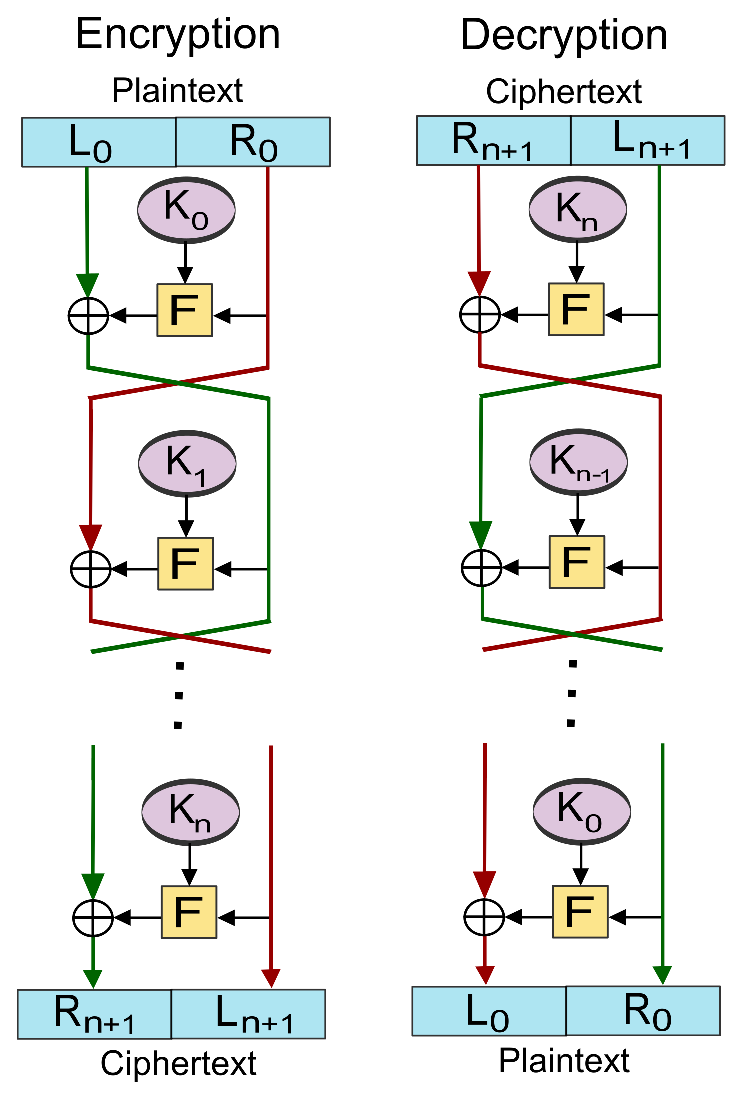
\includegraphics[scale=0.8]{Feistel.eps}
\end{figure}

值得注意到的一点是,在最后一次输出的时候,不再进行交换,也就是说,输出的并不是$\pth{L_{n+1}, R_{n+1}}$, 而是$\pth{R_{n+1}, L_{n+1}}$.
\subsection{SP网络}
SP网络每轮接受到输入之后,首先,将输入与该轮的子密钥进行异或,然后是对输入再次分组(也就是对分过组的明文的每组内容再次进行分组),接着将每个组通过不同的S盒进行代换,代换后的结果再拼成一个新的串,经过一个P盒的置换进行输出。\par
可以通过下图形象地理解SP网络(图源wiki):
\begin{figure}[H]
    \centering
    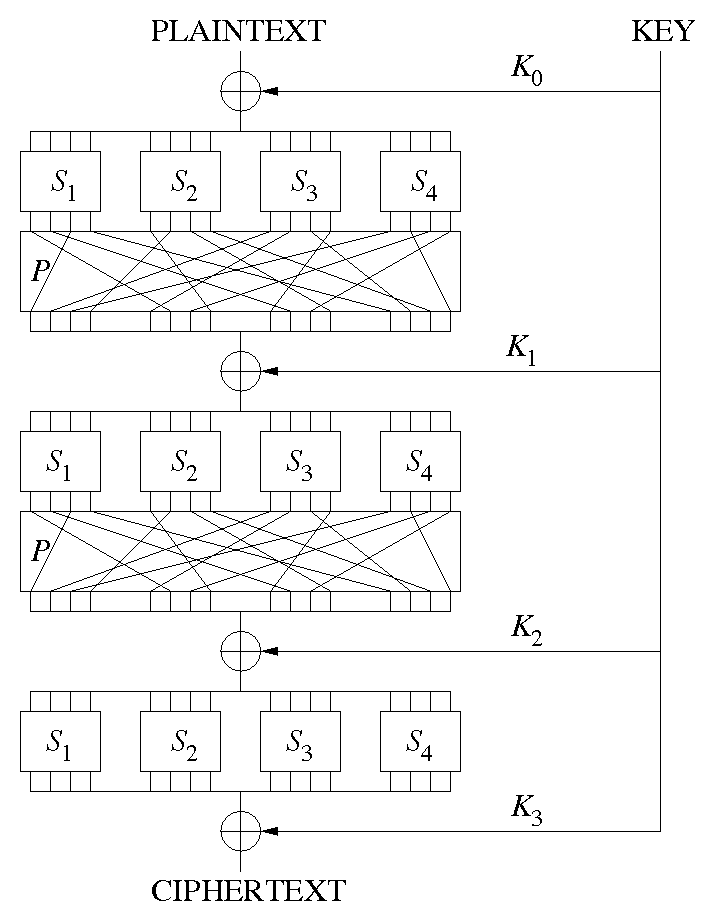
\includegraphics[scale=0.5]{SPN.png}
\end{figure}
\end{document}